\documentclass[uct_visualisation_thesis.tex]{subfiles}

% ------------------- 1. SŁOWNICZEK ---------------------
\chapter{Wykaz najważniejszych oznaczeń i skrótów}
\begin{itemize}
	\item \textbf{MCTS} (Monte Carlo Tree Search) - heurystyka podejmowania decyzji w pewnych zadaniach sztucznej inteligencji, np. ruchów w grach. Najczęściej MCTS opiera się na wariancie metody UCT.
	\item \textbf{UCT} (Upper Confidence Bound Applied to Trees) - algorytm przeszukujący drzewo stanów rozgrywki w poszukiwaniu najbardziej opłacalnych ruchów. Algorytm stara się zachować równowagę między eksploatacją ruchów po ruchach o wysokiej średniej wygranej a eksploracją tych mało sprawdzonych.
	\item \textbf{Podstawowa wizualizacja} - możliwość wyświetlenia całego drzewa stanów. W podstawowej wizualizacji wygląd wierzchołków i krawędzi jest nieistotny.
	\item \textbf{Zaawansowana wizualizacja} - podstawowa wizualizacja wzbogacona o możliwość analizowania statystyk poszczególnych wierzchołków. Kolor wierzchołków będzie reprezentował aktualnego gracza, a kolor krawędzi częstość odwiedzin danego węzła. Możliwe powinno być też przewijanie, przybliżanie oraz oddalanie podglądu drzewa.
	\item \textbf{CSV} - plik w formacie .csv (ang. \textit{comma-separated values}) służący do przechowywania danych w plikach tekstowych, gdzie separatorem jest przecinek.
\end{itemize}

% ------------------- 2. WSTĘP ---------------------
\chapter{Wstęp i cel pracy}
\section{Cel biznesowy}
Algorytm UCT, będący usprawnieniem MCTS, jest powszechnie stosowanym algorytmem w sztucznej inteligencji. Jest metodą analizującą obiecujące ruchy na podstawie generowanego drzewa, która równoważy eksploatację najbardziej korzystnych z eksploracją mniej korzystnych decyzji. Każdemu wierzchołkowi drzewa odpowiada pewien stan rozgrywki, z którego algorytm rozgrywa losowe symulacje, rozszerzając potem drzewo o kolejne możliwe stany. Sposób, w jaki rozrasta się opisywane drzewo, jest kluczowy dla podejmowania przez algorytm jak najlepszych decyzji.\\

Celem projektu jest stworzenie aplikacji pozwalającej na wizualizację drzew algorytmu UCT. Aplikacja będzie pozwalała na wizualizowanie drzew generowanych podczas rozgrywania dwóch przykładowych gier (pozwalając przetestować rozwiązanie). Aplikacja powinna pozwalać na wizualizację drzew, ich sekwencji i róznic między kolejnymi drzewami w sekwencji. Powinna być możliwość płynnego przybliżania/oddalania i przewijania wizualizacji oraz zapisu aktualnego stanu do pliku graficznego - wszystko, aby klient mógł wygodnie korzystać z naszego programu. Taki produkt pozwoliłby zrozumieć klientowi ideę i sposób działania algorytmu UCT.
\section{Założenia projektowe}
\subsection{Założenia funkcjonalne}
Użytkownik korzystający z naszej aplikacji będzie mógł wybrać jedną z dwóch gier deterministycznych, a do wyboru będzie miał trzy tryby rozgrywki:

\begin{enumerate}
	\item Gracz vs PC -- użytkownik będzie decydował o swoich posunięciach i zmierzy się on z zaimplementowanym algorytmem,
	\item PC vs PC -- użytkownik będzie świadkiem symulacji algorytmu, który rozgrywa partię z samym sobą,
	\item Gracz vs Gracz -- rozgrywka dwóch graczy, bez wizualizacji.
\end{enumerate}

Zanim jednak przejdzie do rozgrywki, będzie on miał możliwość ustawienia parametrów algorytmu, tj. liczbę iteracji podczas tworzenia drzewa, czy też maksymalny czas na ruch przeciwnika.
Druga opcja, którą będzie dysponować użytkownik, to możliwość wczytania drzewa w formacie zarówno binarnym jak i CSV, a następnie możliwość jego dogłębnej analizy. Będzie on mógł wyświetlać informacje na temat wybranego węzła, a także przybliżać i oddalać całą wygenerowaną strukturę. Podczas samej rozgrywki, po wykonanym ruchu przeciwnika gracz będzie mógł analizować drzewo w sposób opisany powyżej, a także wyeksportować je. Będzie też miał możliwość zapisania go w wyżej wymienionych formatach, a także w formacie rastrowym. Użytkownik będzie mógł oglądać animację rozrostu drzewa. Powyższe rzeczy dotyczą trybów gry z udziałem algorytmu i każdej z gier.\\

Aplikacja będzie potrzebować procesora graficznego. Dostęp do sieci nie jest potrzebny dla poprawnego działania aplikacji. \\

Diagram przypadków użycia, który ilustruje przedstawione możliwości, znajduje się na rysunku \ref{rys:usecase}.
\begin{figure}[h!]
	\centering
	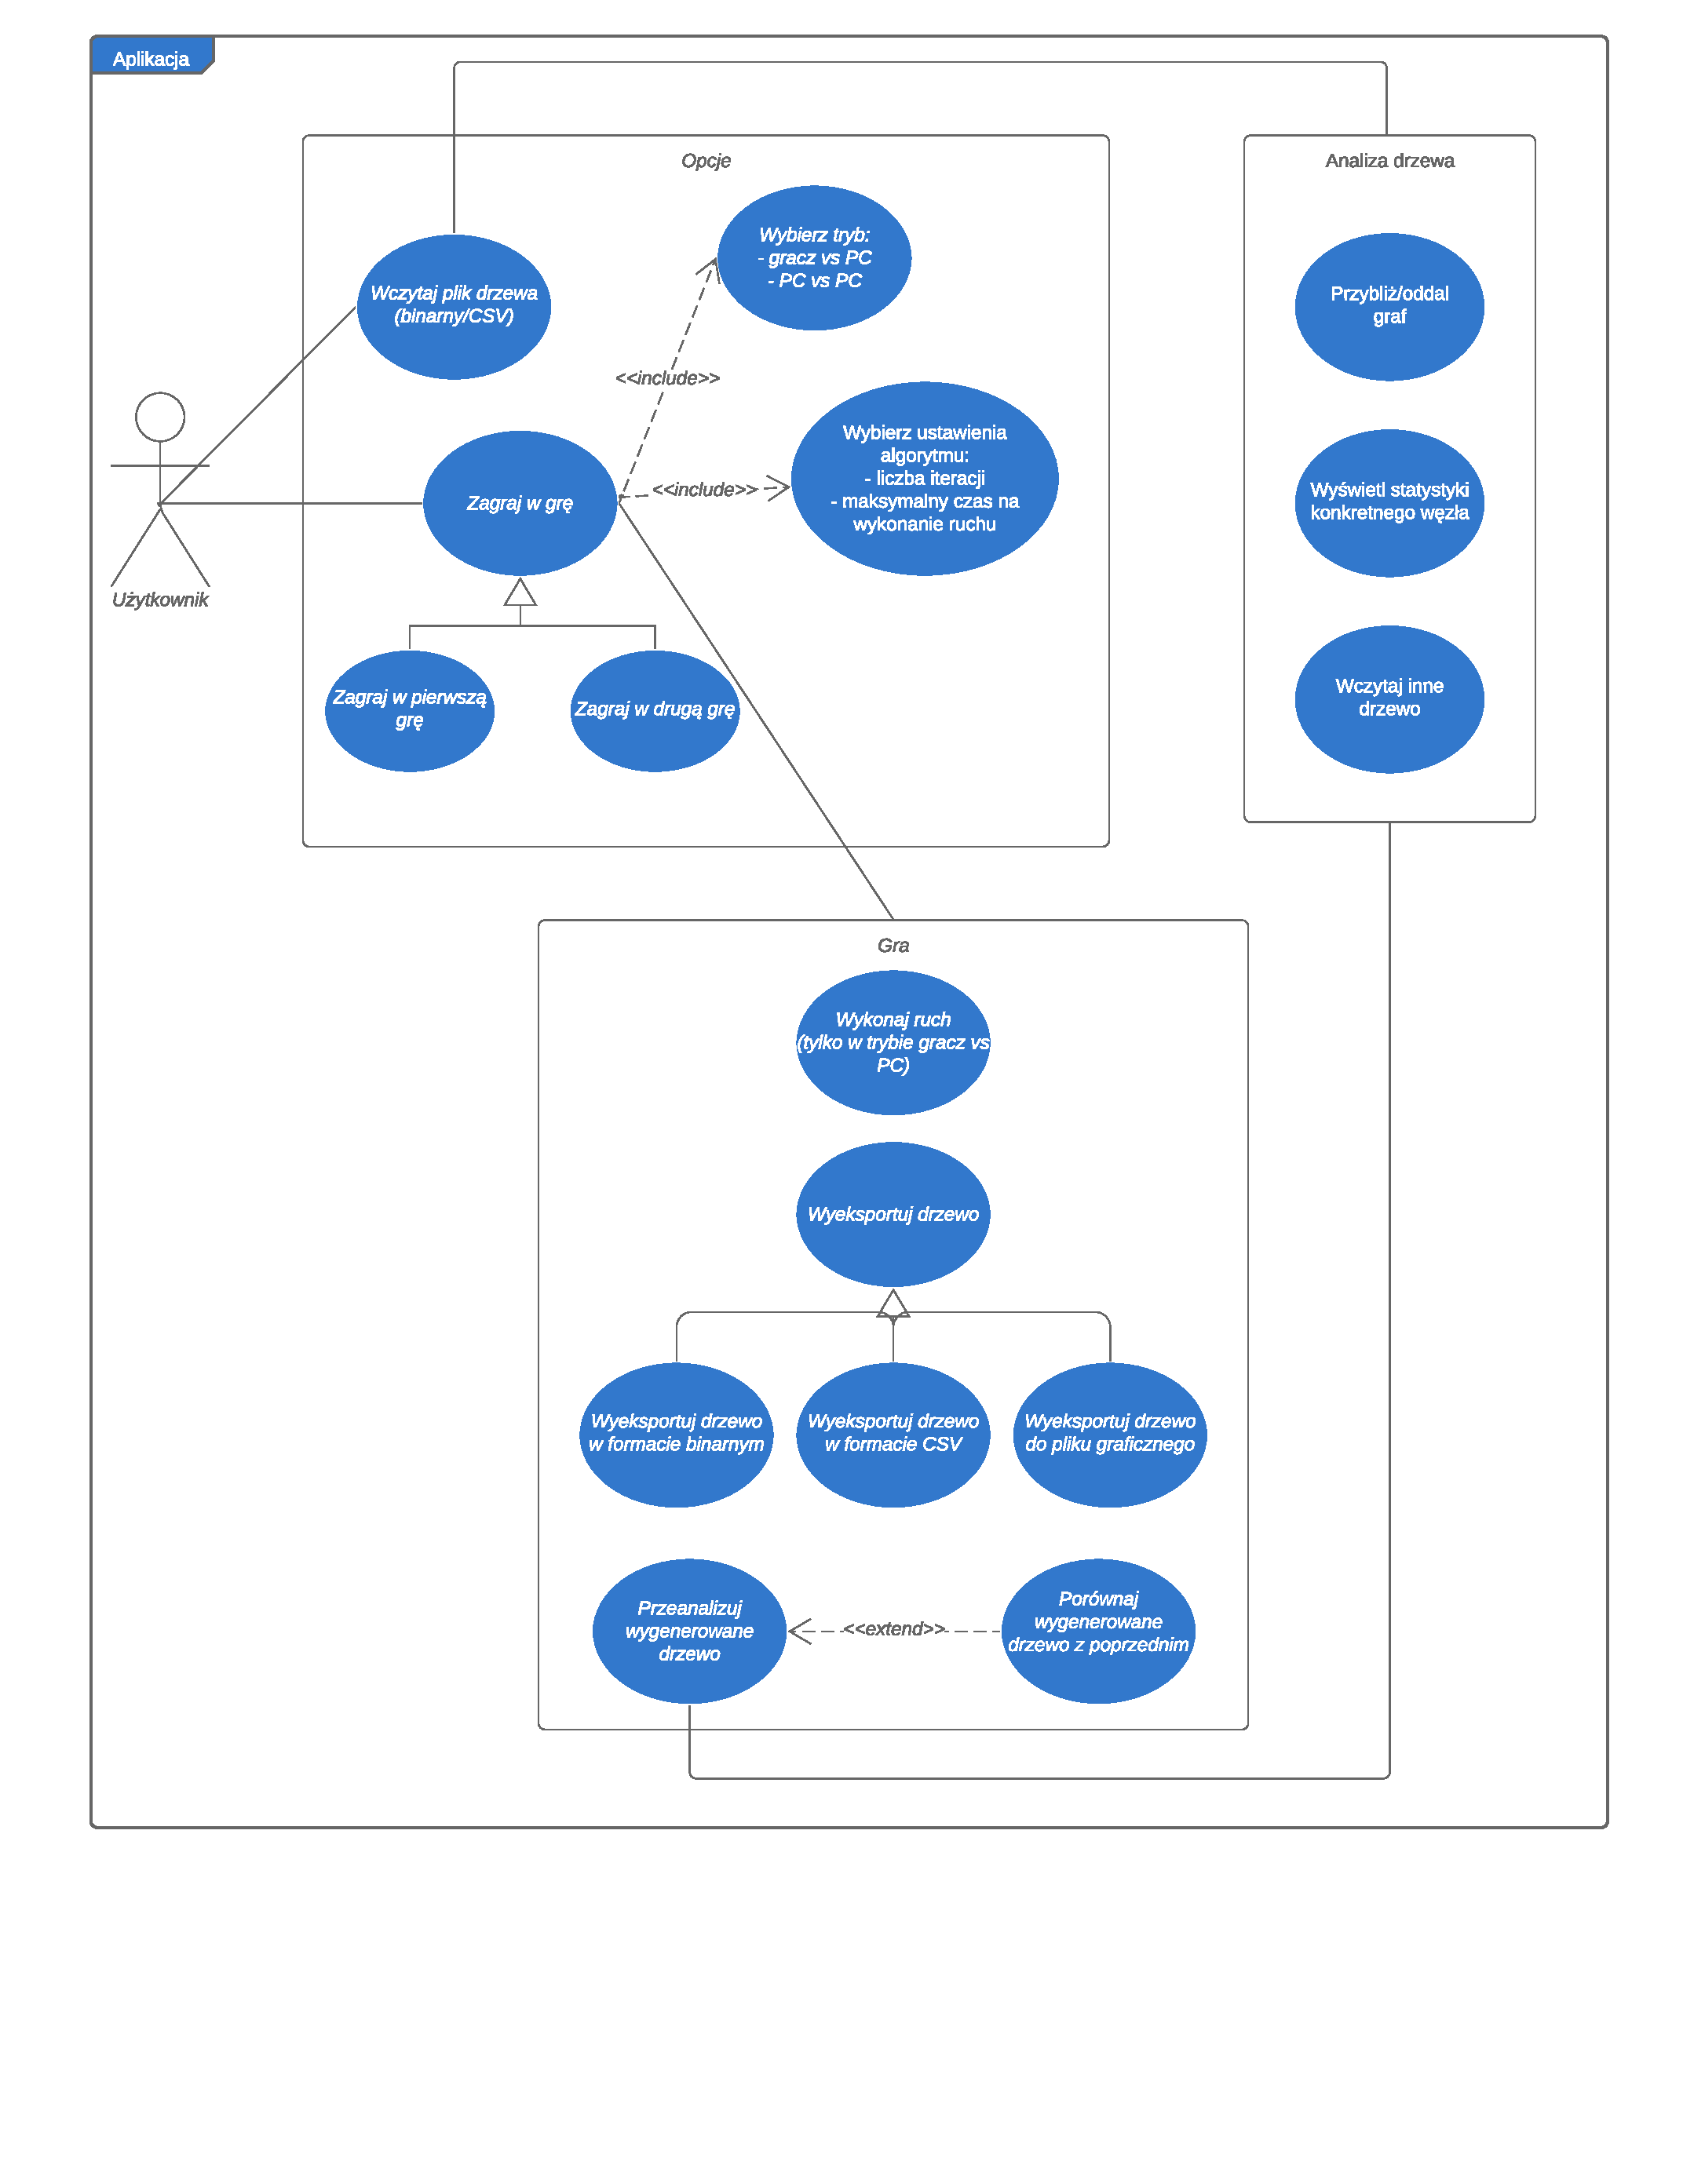
\includegraphics[width=\textwidth, trim={0 6.5cm 0 0},clip]{aplikacja-use-case-eps}
	\caption{Diagram przypadków użycia}
	\label{rys:usecase}
\end{figure}

\subsection{Założenia niefunkcjonalne}
Wymagania niefunkcjonalne opisane są w tabeli \ref{tab:furps} przy użyciu metody FURPS. Zawiera ona między innymi opis wymagań sprzętowych aplikacji oraz jej ograniczenia wydajnościowe.

\begin{table}[h!]
	\caption{Analiza FURPS}
	\label{tab:furps}
	\centering
	\begin{tabular}{|l|p{0.7\linewidth}|}
		\hline
		Obszar         & \textbf{Opis} \\ \hline
		Używalność     & Aplikacja działa w jednym oknie wyposażonym w przejrzysty interfejs dla użytkownika. Ponadto, dostarczona jest instrukcja instalacji i obsługi programu.  \\ \hline
		Niezawodność   & Aplikacja działa na komputerze lokalnym i po zainstalowaniu jest dostępna cały czas. Potencjalne błędy nie powinny zamykać aplikacji, a jedynie wyświetlić komunikat dla użytkownika.\\ \hline
		Wydajność      & Aplikacja koryszta głównie z pamięci RAM, procesora i procesora graficznego. Dla drzew do 100 000 wierzchołków wizualizacja nie powinna zajmować więcej niż 3s, a dla 250 000 ---  5s. Wszystkie obliczenia i wizualizacje są przeprowadzane wewnątrz jednej maszyny.\\ \hline
		Wsparcie       & Aplikacja jest przeznaczona dla komputerów z systemami operacyjnymi Windows oraz Linux. \\ \hline
	\end{tabular}
\end{table}

% ------------------- 3. TEORIA ---------------------
\chapter{Teoria}
\section{Algorytmy MCTS}
\textbf{MCTS} (Monte Carlo Tree Search) - heurystyka podejmowania decyzji w pewnych zadaniach sztucznej inteligencji, np. ruchów w grach. Najczęściej MCTS opiera się na jakimś wariancie metody UCT.

\subsection{Opis grupy algorytmów}
Algorytm jest opisany w formie pseudokodu w listingu \ref{lst:mcts}. Nasza implementacja będzie oparta o \cite{banditbased}.\\

Algorytm Monte Carlo Tree Search opiera się na rozbudowywaniu drzewa ze stanami gry, poprzez iteracyjne wykonywanie czterech faz, opisanych poniżej.
\begin{enumerate}
	\item \textbf{Faza wyboru} (linia 6 w listingu) - wybranie najbardziej obiecującego wierzchołka do rozrostu drzewa. Istotny w tej fazie jest balans pomiędzy eksploracją ruchów przeanalizowanych najdokładniej oraz eksploatacją jeszcze niezbadanych.
	\item \textbf{Faza rozrostu} (linia 7 w listingu) - utworzenie wierzchołków potomnych dla najbardziej obiecującego wierzchołka. Tworzone wierzchołki odpowiadają stanom możliwym do uzyskania poprzez wykonanie jednego ruchu ze stanu wierzchołka obiecującego.
	\item \textbf{Faza symulacji} (linia 8 w listingu) - rozegranie losowej rozgrywki ze stanu jednego z utworzonych wierzchołków utworzonych w poprzedniej fazie.
	\item \textbf{Faza propagacji wstecznej} (linia 9 w listingu) - aktualizacja informacji wierzchołków na ścieżce od wierzchołka, z którego rozpoczęto symulację, do korzenia drzewa.
\end{enumerate}

\begin{lstlisting}[caption={Pseudokod algorytmu Monte Carlo Tree Search}, label=lst:mcts, style=mystyle]
def find_next_move(curr_state):
	iterations_counter = 0
	tree = initialize_tree(curr_state)
	
	while iterations_counter < max_iterations_counter:
		# selection(tree.root) 
		curr_node = select promising node based on UCT formula      
		
		# expansion(node)
		create child nodes from node
		
		# simulation(node)		
		playout_result = simulate random playout from curr_node     
		
		# backpropagation(node, playout_result)
		update tree according to playout_result                     
		
		iterations_counter++
	
	best_state = select best child(tree.root) 
	return best_state
\end{lstlisting}

\section{Algorytm UCT}
\textbf{UCT} (Upper Confidence Bound Applied to Trees) - algorytm przeszukujący drzewo stanów rozgrywki w poszukiwaniu najbardziej opłacalnych ruchów. Algorytm stara się zachować równowagę między eksploatacją ruchów po ruchach o wysokiej średniej wygranej a eksploracją tych mało sprawdzonych.

\subsection{Opis algorytmu}
Moduł \textbf{Algorytm} jest implementacją algorytmu Monte Carlo Tree Search, korzystającą z wariantu UCT. Odpowiedzialnością tego modułu jest wyznaczanie kolejnego ruchu na podstawie dostarczonego stanu gry. Opisywany moduł będzie odpowiadał za iteracyjne tworzenie drzewa stanów i przeszukiwanie go w celu wyznaczenia najbardziej korzystnego ruchu. Użytkownik będzie miał możliwość zmiany liczby iteracji algorytmu albo ograniczenie czasowe jego działania.\\

W listingu \ref{lst:mcts} operujemy na trzech istotnych zmiennych - \textbf{tree}, \textbf{curr\textunderscore node} i \textbf{curr\textunderscore state}. Odpowiedzialnością struktury opisującej \textbf{tree} jest przechowywanie korzenia drzewa oraz stanu wyjściowego rozgrywki, który jest tej samej struktury co zmienna \textbf{curr\textunderscore state}. Struktura opisująca \textbf{curr\textunderscore node} przechowuje wszystkie informacje na temat wierzchołka drzewa, wraz z referencjami do wierzchołków potomnych i rodzica.

\subsection{Dodatkowe założenia}
Aby gra była poprawnie obsłużona przez utworzony system, musi spełniać następujące założenia:

\begin{enumerate}
	\item Rozgrywka jest prowadzona naprzemiennie przez dwóch graczy.
	\item Każdy ruch ma jednoznaczny wpływ na dalszą rozgrywkę (rozgrywka jest deterministyczna).
	\item Każdy z graczy ma dostęp do pełnej informacji o aktualnym stanie gry.
\end{enumerate}

\section{Algorytm wizualizacji drzewa}
\subsection{Określenie problematyki}
\subsection{Założenia}
Aby wizualizacja była czytelna, poczyniliśmy następujące założenia:
\begin{enumerate}
	\item Krawędzie drzewa nie mogą się przecinać.
	\item Wierzchołki będą ustawione od góry w rzędach, a przynależność do
	rzędów będzie zależała od odległości wierzchołków od korzenia.
	\item Wierzchołki mają być narysowane możliwie najwęziej.
\end{enumerate}


\subsection{Usprawniony algorytm Walkera}
Aby wyznaczyć układ wierzchołków na płaszczyźnie, spełniając powyższe 3 założenia, skorzystamy z usprawnionego algorytmu Walkera, który działa w czasie liniowym względem liczby wierzchołków. Algorytm, który zaimplementujemy, został opisany w \cite{impwalkers}.


% ------------------- 4. IMPLEMENTACJA ---------------------
\chapter{Implementacja}
\section{Wykorzystane technologie}
W naszym projekcie zdecydowaliśmy się skorzystać z:
\begin{enumerate}
	\item Języka \textit{Python} w wersji 3.7.2.
	\item Biblioteki \textit{VisPy} w wersji 0.6.3, która udostępnia komponenty związane z wizualizacją graficzną. Wykorzystujemy tę bibliotekę w połączeniu z \textit{OpenGL} w wersji 2.1. Biblioteka \textit{VisPy} jest stworzona w oparciu o licencję \textit{BSD}, co w kontekście projektu na pracę inżynierską pozwala na modyfikowanie i wykorzystywanie jej.
	\item Nakładki na bibliotekę Qt - \textit{PyQt5} w wersji 5.9.2. \textit{PyQt5} umożliwia tworzenie interfejsu graficznego. Dla projektów takich jak praca inżynierska, \textit{PyQt} dystrybuowana jest na zasadach \textit{GNU General Public License}.
	\item Biblioteki \textit{fman build system (fbs)} w wersji 0.8.4, ułatwiającej pakowanie aplikacji w języku \textit{Python} korzystających z biblioteki \textit{PyQt}. To oprogramowanie dystrybuowane jest na zasadach \textit{GNU General Public License}.
	\item Narzędzia \textit{pdoc} w wersji 0.3.2, służącego do automatycznego generowania dokumentacji aplikacji.
\end{enumerate}


\section{Architektura i działanie systemu}
Aplikacja będzie podzielona na pięć oddzielnych modułów: \textit{algorytm}, \textit{serializacja}, \textit{wizualizacja}, \textit{gry}, które będą funkcjonować w obrębie nadrzędnego modułu - \textit{aplikacji głównej}. Cele każdego z modułów i zadania powierzone im są przedstawione poniżej.

\subsection{Algorytm}
\subsection{Serializacja}
\subsection{Wizualizacja}
\subsection{Gry}
\subsection{Aplikacja główna}

\section{Główne komponenty aplikacji}
\section{Interfejs użytkownika}


% ------------------- 5. INSTRUKCJE ---------------------
\chapter{Instrukcje}
\section{Instrukcja instalacji}
\section{Instrukcja użytkownika}


% ------------------- 6. OCENA I PODSUMOWANIE---------------------
\chapter{Podsumowanie i ocena}
\section{Uzyskane efekty}
\section{Kontynuacja pracy}
\section{Wydajność}
\section{Testy akceptacyjne}
Testy akceptacyjne zostały przeprowadzone w celu sprawdzenia, czy aplikacja spełnia założenia opisane w dokumentacji wymagań projektu. Test \ref{tab:test1} konfrontuje założenia modułu \textit{Gry}, test \ref{tab:test2} – modułu \textit{Serializacja}, a pozostałe testy weryfikują założenia modułu \textit{Wizualizacja}.\\

Testy akceptacyjne zostały wykonane na komputerze:

\begin{itemize}
	\item z zainstalowanym systemem operacyjnym \textit{Windows 10 Education N},
	\item z zainstalowanym interpreterem języka \textit{Python 3.7.2} i biblioteką \textit{PyQt5},
	\item wyposażonym w procesor \textit{Intel Core i7-8700k @3.70 GHz},
	\item wyposażonym w kartę graficzną \textit{NVIDIA GeForce GTX 1060 6GB},
	\item wyposażonym w 32GB pamięci RAM.
\end{itemize}

Pierwszy z przeprowadzonych testów dotyczy funkcjonalności modułu \textit{Gry}, a wynik opisany został w tabeli \ref{tab:test1}.

\begin{table}[H]
	\caption{Raport z pierwszego testu}
	\label{tab:test1}
	\centering
	\begin{tabular}{|c|p{0.6\textwidth}|}
		\hline
		Testowane wymaganie & \textit{Użytkownik będzie mógł wybrać jedną z dwóch przykładowych gier, a do wyboru będzie miał trzy tryby rozgrywki.} \\ \hline
		Kroki testowe & \begin{enumerate} \item Z menu głównego aplikacji wybierz opcję \textit{Chess}. \item Z menu głównego aplikacji wybierz opcję \textit{Player vs player} i sprawdź tryb rozgrywki dla dwóch graczy. \item Z menu głównego aplikacji wybierz opcję \textit{Player vs PC} dla różnych ustawień algorytmu UCT. \item Z menu głównego aplikacji wybierz opcję \textit{PC vs PC} dla różnych ustawień algorytmu UCT. \item Z menu głównego aplikacji wybierz \textit{Mancala} i powtórz kroki 2–5. \end{enumerate} \\ \hline
		Wynik & Pozytywny. \\ \hline
	\end{tabular}
\end{table}

Drugi z przeprowadzonych testów dotyczy funkcjonalności modułu \textit{Serializacja}, a wynik opisany został w tabeli \ref{tab:test2}.

\begin{table}[H]
	\caption{Raport z drugiego testu}
	\label{tab:test2}
	\centering
	\begin{tabular}{|c|p{0.6\textwidth}|}
		\hline
		Testowane wymaganie & \textit{Użytkownik będzie mógł zapisać analizowane drzewa do pliku csv, do pliku binarnego oraz do bitmapy.} \\ \hline
		Kroki testowe & \begin{enumerate} \item Z menu głównego aplikacji wybierz ścieżkę do dowolnego pliku z zserializowanym drzewem. \item Naciśnij przycisk \textit{Inspect tree}. \item Naciśnij przycisk \textit{Save to csv file}. \item Naciśnij przycisk \textit{Save to binary file}. \item Naciśnij przycisk \textit{Save to bitmap file}. \item Sprawdź, czy bitmapa wygenerowana w kroku 5 odpowiada drzewu z pliku początkowego. \item Z menu głównego aplikacji wybierz ścieżkę plików wygenerowanych w kroku 3 i 4, żeby sprawdzić, czy zapisane drzewa wizualizowane są tak samo jak w początkowym pliku. \end{enumerate} \\ \hline
		Wynik & Pozytywny. \\ \hline
	\end{tabular}
\end{table}

Trzeci z przeprowadzonych testów dotyczy funkcjonalności modułu \textit{Wizualizacja}, a wynik opisany został w tabeli \ref{tab:test3}.

\begin{table}[H]
	\caption{Raport z trzeciego testu}
	\label{tab:test3}
	\centering
	\begin{tabular}{|c|p{0.6\textwidth}|}
		\hline
		Testowane wymaganie & \textit{Użytkownik będzie mógł wyświetlić informacje związane z wybranym węzłem drzewa, a także przybliżać i oddalać cały graf.} \\ \hline
		Kroki testowe & \begin{enumerate} \item Z menu głównego aplikacji wybierz ścieżkę do dowolnego pliku z drzewem. \item Naciśnij przycisk \textit{Inspect tree}. \item Przy użyciu prawego przycisku myszki chwyć za obszar rysowania i poruszaj się po wizualizacji. \item Używając kółka myszki, przybliż i oddal wizualizowane drzewo. \item Kliknij dowolny wierzchołek drzewa lewym przyciskiem myszki i sprawdź, czy panel z prawej strony wyświetla informacje związane z wybranym wierzchołkiem. \end{enumerate} \\ \hline
		Wynik & Pozytywny. \\ \hline
	\end{tabular}
\end{table}

Czwarty z przeprowadzonych testów dotyczy wydajności modułu \textit{Wizualizacja}, a wynik opisany został w tabeli \ref{tab:test4}.

\begin{table}[H]
	\caption{Raport z czwartego testu}
	\label{tab:test4}
	\centering
	\begin{tabular}{|c|p{0.6\textwidth}|}
		\hline
		Testowane wymaganie & \textit{Dla drzew do 100 000 wierzchołków wizualizacja nie powinna zajmować więcej niż 3s.} \\ \hline
		Kroki testowe & \begin{enumerate} \item Z menu głównego aplikacji wybierz ścieżkę do pliku \textit{tree\textunderscore 100k.csv}. \item Naciśnij przycisk \textit{Inspect tree}. \end{enumerate} \\ \hline
		Wynik & Pozytywny – deserializacja, ulepszony algorytm Walkera i wyświetlenie drzewa z pliku zajęło 2.802s. \\ \hline
	\end{tabular}
\end{table}

Piąty z przeprowadzonych testów dotyczy wydajności modułu \textit{Wizualizacja}, a wynik opisany został w tabeli \ref{tab:test5}.

\begin{table}[H]
	\caption{Raport z piątego testu}
	\label{tab:test5}
	\centering
	\begin{tabular}{|c|p{0.6\textwidth}|}
		\hline
		Testowane wymaganie & \textit{Dla drzew do 250 000 wierzchołków wizualizacja nie powinna zajmować więcej niż 5s.} \\ \hline
		Kroki testowe & \begin{enumerate} \item Z menu głównego aplikacji wybierz ścieżkę do pliku \textit{tree\textunderscore 250k.csv}. \item Naciśnij przycisk \textit{Inspect tree}. \end{enumerate} \\ \hline
		Wynik & Pozytywny – deserializacja, ulepszony algorytm Walkera i wyświetlenie drzewa z pliku zajęło 4.626s. \\ \hline
	\end{tabular}
\end{table}

Wszystkie testy akceptacyjne zakończyły się pozytywnie, a więc wymagania zostały spełnione.

% ------------------- 6. WNIOSKI ---------------------
\chapter{Wnioski}
